\documentclass[10pt, aspectratio=169]{beamer}

\usetheme{metropolis}
\metroset{progressbar=none, sectionpage=progressbar}

\usepackage{listings}
\usepackage{xcolor}
\usepackage{booktabs}
\usepackage{tikz}
\usetikzlibrary{arrows.meta, positioning, fit, backgrounds}

% ---------------------------------------------------------------- code style
\definecolor{cmt}{HTML}{6E7B8B}
\definecolor{kw}{HTML}{1F6FEB}
\definecolor{ssa}{HTML}{8250DF}
\definecolor{bg}{HTML}{F6F8FA}

\lstdefinestyle{mlir}{
  basicstyle=\ttfamily\scriptsize,
  keywordstyle=\color{kw},
  commentstyle=\color{cmt}\itshape,
  morecomment=[l]{//},
  morecomment=[l]{\#},
  keywords={scf.for,scf.yield,linalg.generic,linalg.elementwise,tensor.extract_slice,
            tensor.insert_slice,iter_args,ins,outs,step,to,transform.structured.match,
            transform.split_handle,transform.annotate,transform.get_producer_of_operand,
            transform.structured.fuse_dependant_reduction_ops,
            transform.structured.tile_using_for,for,if,def},
  showstringspaces=false,
  columns=fullflexible,
  keepspaces=true,
  breaklines=false,
  backgroundcolor=\color{bg},
  frame=none,
  xleftmargin=2pt,
  aboveskip=2pt,
  belowskip=2pt,
}
\lstset{style=mlir}
\newcommand{\code}[1]{\texttt{\small #1}}

% ---------------------------------------------------------------- title page
% Background is page 1 of slides_template.pdf with its text stripped.
\definecolor{inteltitle}{HTML}{0068B5}
\definecolor{intelsub}{HTML}{004A86}
\setbeamertemplate{title page}{%
  \vfill
  \begin{center}
    {\color{inteltitle}\fontsize{22}{27}\selectfont\inserttitle\par}
    \ifx\insertsubtitle\empty\else
      \vspace{2mm}
      {\color{intelsub}\large\insertsubtitle\par}
    \fi
    \vspace{6mm}
    {\color{intelsub}\large\insertauthor\par}
    \vspace{1mm}
    {\color{intelsub}\normalsize\insertdate\par}
  \end{center}
  \vfill
}
\makeatletter
\renewcommand{\maketitle}{%
  \begingroup
    \setbeamertemplate{background}{%
      
\includegraphics[width=\paperwidth,height=\paperheight]{title_bg.pdf}}
    \begin{frame}[plain,noframenumbering]
      \usebeamertemplate{title page}
    \end{frame}
  \endgroup
}
\makeatother

% ------------------------------------------------------------ content slides
% Background is page 4 of slides_template.pdf with its text stripped:
% gray strips along the bottom (6mm) and right (6mm) edges, Intel logo in the
% bottom strip and a white corner square for the slide number.
\definecolor{intelgray}{HTML}{525252}
\setbeamertemplate{background}{%
  
\includegraphics[width=\paperwidth,height=\paperheight]{content_bg.pdf}}
\setbeamersize{text margin left=6.2mm, text margin right=8.5mm}
\setbeamercolor{normal text}{fg=intelgray}
\setbeamercolor{frametitle}{fg=intelgray, bg=}
\setbeamercolor{alerted text}{fg=inteltitle}
\setbeamercolor{progress bar}{fg=inteltitle, bg=inteltitle!15}
\setbeamercolor{section title}{fg=intelgray}
\setbeamerfont{frametitle}{size=\LARGE, series=\normalfont}
\setbeamertemplate{frametitle}{%
  \nointerlineskip
  \begin{beamercolorbox}[wd=\paperwidth, leftskip=6.2mm, rightskip=8.5mm]{frametitle}
    \rule{0pt}{10mm}\insertframetitle\rule[-2.5mm]{0pt}{2.5mm}
  \end{beamercolorbox}%
}
\setbeamertemplate{itemize item}{\raisebox{0.3ex}{\rule{0.6ex}{0.6ex}}}
\setbeamertemplate{itemize subitem}{\raisebox{0.35ex}{\rule{0.4ex}{0.4ex}}}
% Slide number centered in the bottom-right white square.
\setbeamertemplate{footline}{%
  \vbox to 6mm{\vfill
    \hbox to \paperwidth{\hfill
      \makebox[6mm][c]{\fontsize{5}{6}\selectfont\color{intelgray}\insertframenumber}}%
    \vskip 2.2mm}%
}

\title{An Approach for Tiling and Fusing \\Dependent Reductions in Linalg}
% \subtitle{A composable Transform primitive with automatic online correction}
\date{8/26/2026 }
\author{Charitha Saumya}

\begin{document}

\maketitle

% =============================================================== Motivation
\begin{frame}[fragile]{The pattern: dependent reductions (softmax)}
  Two reductions over the \alert{same} axis \code{j}, the second depending on the
  first:
  \[
    m = \max_j x[j] \qquad\longrightarrow\qquad s = \sum_j \exp(x[j] - m)
  \]
  \vspace{-2mm}
  \begin{columns}[t]
    \begin{column}{0.48\textwidth}
      \textbf{Two passes over \code{x}}
\begin{lstlisting}
// pass 1
for j: m = max(m, x[j])
// pass 2: re-reads x, needs full m
for j: s += exp(x[j] - m)
\end{lstlisting}
      \begin{itemize}\small
        \item intermediate materialized
        \item $2\times$ memory traffic
      \end{itemize}
    \end{column}
    \begin{column}{0.48\textwidth}
      \textbf{One online pass}
\begin{lstlisting}
for j:
  m_new = max(m, x[j])
  // online correction
  s = s * exp(m - m_new)
      + sum(exp(x[j] - m_new))
  m = m_new
\end{lstlisting}
      \begin{itemize}\small
        \item accumulators stay in registers
        \item the basis of flash attention
      \end{itemize}
    \end{column}
  \end{columns}
\end{frame}

\begin{frame}{What Linalg gives us today}
  \begin{columns}[t]
    \begin{column}{0.48\textwidth}
      \textbf{Available today}
      \begin{itemize}\small
        \item Tile and fuse producer--consumer chains along \emph{parallel} dims\\
          {\scriptsize\code{tile\_using\_for} + \code{fuse\_into\_containing\_op}}
        \item Tile a \emph{single} reduction along its reduction dim\\
          {\scriptsize\code{tile\_using\_for} with \code{FullReduction}}
      \end{itemize}
    \end{column}
    \begin{column}{0.48\textwidth}
      \textbf{\alert{Missing}}
      \begin{itemize}\small
        \item Fusing \emph{dependent} reductions that share a reduction axis
        \item Each reduction becomes its own loop; the intermediate is
          materialized and re-read
        \item Requires \alert{online correction}: when the producer's running
          accumulator changes, partial results of the dependent reduction must be
          rescaled
      \end{itemize}
    \end{column}
  \end{columns}

  \vspace{4mm}
  \small Today that knowledge lives in hand-written kernels, monolithic
  high-level ops, or bespoke pattern-matching passes --- not in a reusable
  Linalg primitive.
\end{frame}

% =============================================================== Key idea
\begin{frame}{When can we fuse? The factorizability condition}
  Chain: \quad \code{R1} (reduction) $\rightarrow$ \code{E} (elementwise term)
  $\rightarrow$ \code{R2} (reduction)
  \vspace{2mm}
  \begin{itemize}
    \item \code{R2} must be a \alert{sum} reduction, and \code{R1} must enter each
      summed term \code{E} in a \alert{factorizable (i.e. multiplicatively separable)} way.
    \item Softmax: \; $\exp(x - m) = \underbrace{\exp(x)}_{\text{data}} \cdot
      \underbrace{\exp(-m)}_{\text{depends on } R1}$
    \item Distributivity of $\cdot$ over $+$ $\Rightarrow$ a stale accumulator can
      be repaired by \emph{rescaling} it:
      \[
        \text{acc}' = \text{acc} \cdot
        \frac{E'(m_{\text{new}})}{E'(m_{\text{old}})}
        \;=\; \text{acc}\cdot \exp(m_{\text{old}} - m_{\text{new}})
      \]
    \item Also covers a contraction consumer (\code{P @ V}): \code{E} is one of the
      matmul operands.
  \end{itemize}
\end{frame}

\begin{frame}{Deriving the correction automatically from \code{E}}
  \centering
  \resizebox{\textwidth}{!}{%
  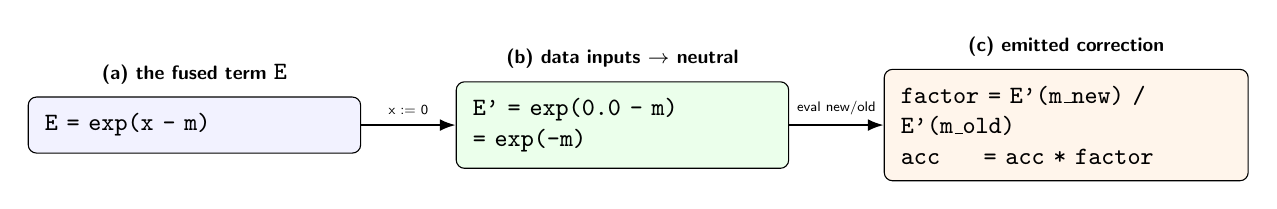
\begin{tikzpicture}[
      font=\ttfamily\small,
      box/.style={draw, rounded corners=3pt, align=left, inner sep=6pt,
                  fill=black!3, text width=38mm},
      stlbl/.style={font=\sffamily\scriptsize\bfseries},
      arr/.style={-{Latex[length=2mm]}, thick},
    ]
    \node[box, fill=blue!5] (b1) {E = exp(x - m)};
    \node[stlbl, above=1pt of b1] {(a) the fused term \code{E}};

    \node[box, right=12mm of b1, fill=green!8] (b2) {E' = exp(0.0 - m)\\= exp(-m)};
    \node[stlbl, above=1pt of b2] {(b) data inputs $\rightarrow$ neutral};

    \node[box, right=12mm of b2, fill=orange!8, text width=42mm] (b3)
      {factor = E'(m\_new) / E'(m\_old)\\acc \ \ \ \ = acc * factor};
    \node[stlbl, above=1pt of b3] {(c) emitted correction};

    \draw[arr] (b1) -- (b2) node[midway, above, font=\sffamily\tiny] {x := 0};
    \draw[arr] (b2) -- (b3) node[midway, above, font=\sffamily\tiny] {eval new/old};
  \end{tikzpicture}}

  \vspace{3mm}
  \begin{itemize}\small
    \item Clone \code{E}'s body, replace every \emph{data} input by the constant
      that eliminates it at its use point (\code{0} for \code{add}/\code{sub},
      \code{1} for \code{mul}/\code{div}).
    \item Sound because data inputs cancel in the ratio:
      $\exp(x-m_{\text{new}})/\exp(x-m_{\text{old}})$ is independent of $x$.
    \item Softmax gets exactly the flash-attention rescale --- \emph{emitted}, not
      hard-coded.
  \end{itemize}
\end{frame}

% =============================================================== Proposed op
\begin{frame}[fragile]{Proposed op: \code{structured.fuse\_dependant\_reduction\_ops}}
  Three operand handles, one result:
  \begin{enumerate}\small
    \item \textbf{\code{R1}} --- already tiled producer reduction
      (\code{scf.for} from \code{tile\_using\_for} with \code{FullReduction},
      accumulator carried as \code{iter\_arg}; may carry several results).
    \item \textbf{\code{E}} --- all-parallel elementwise op consuming an \code{R1}
      result as a broadcast input.
    \item \textbf{\code{R2}} --- still-untiled consumer reduction over the same
      axis, reducing \code{E}'s result.
  \end{enumerate}
  \vspace{1mm}
\begin{lstlisting}
%loop = ..... -> !transform.any_op   // R1: the already tiled reduction loop
%e    = ..... -> !transform.any_op   // E : the elementwise term
%r2   = ..... -> !transform.any_op   // R2: the consumer reduction

%fused = transform.structured.fuse_dependant_reduction_ops %e, %r2 into %loop
    : (!transform.any_op, !transform.any_op, !transform.any_op)
    -> !transform.any_op
\end{lstlisting}
  \vspace{1mm}
  \small Returns the loop, now also carrying \code{E} and \code{R2}, fused and
  online $\Rightarrow$ \alert{apply repeatedly} for chains of dependent reductions.
\end{frame}

\begin{frame}{Main stages of the transformation}
  \centering
  \resizebox{\textwidth}{!}{%
  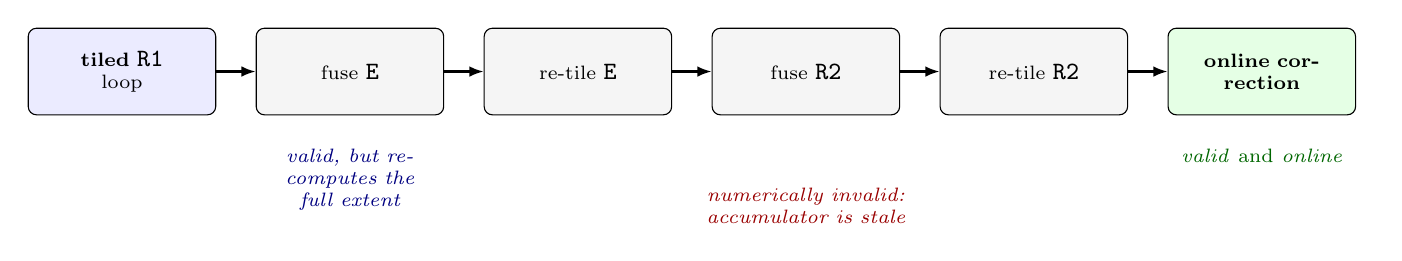
\begin{tikzpicture}[
      font=\scriptsize,
      st/.style={draw, rounded corners=3pt, fill=black!4, text width=21mm,
                 align=center, inner sep=4pt, minimum height=11mm},
      arr/.style={-{Latex[length=1.8mm]}, thick},
      note/.style={font=\scriptsize\itshape, align=center},
    ]
    \node[st, fill=blue!8] (s0) {\textbf{tiled \code{R1}}\\loop};
    \node[st, right=5mm of s0] (s1) {fuse \code{E}};
    \node[st, right=5mm of s1] (s2) {re-tile \code{E}};
    \node[st, right=5mm of s2] (s3) {fuse \code{R2}};
    \node[st, right=5mm of s3] (s4) {re-tile \code{R2}};
    \node[st, right=5mm of s4, fill=green!10] (s5) {\textbf{online correction}};

    \foreach \a/\b in {s0/s1, s1/s2, s2/s3, s3/s4, s4/s5}
      \draw[arr] (\a) -- (\b);

    \node[note, below=3mm of s1, text width=24mm, text=blue!50!black]
      {valid, but recomputes the full extent};
    \node[note, below=8mm of s3, text width=30mm, text=red!60!black]
      {numerically invalid: accumulator is stale};
    \node[note, below=3mm of s5, text width=26mm, text=green!40!black]
      {valid \emph{and} online};
  \end{tikzpicture}}

  \vspace{4mm}
  \begin{itemize}\small
    \item One op at a time, \code{E} first: \emph{fuse} (\code{scf::tileAndFuseConsumer}),
      then immediately \emph{re-tile} to \code{R1}'s tile.
    \item \code{E} first, so \code{R2} is fused against the slice \code{E} yields.
    \item Implemented as an \code{OpRewritePattern} on \code{R2}; a control function
      confines fusion to the handles named by the transform op.
  \end{itemize}
\end{frame}

% =============================================================== Example
\section{Example: standard attention $\rightarrow$ fused attention}

\begin{frame}{The attention chain}
  Score matrix \code{x = Q @ K\textsuperscript{T}}, values \code{V}; all
  reductions over the key axis \code{j}. Normalization is deferred
  (flash-attention-v2):
  \vspace{1mm}
  \[
  \begin{aligned}
    R1 \;(\max):&\quad m[i]    = \max_j x[i,j] \\
    E \;(\text{term}):&\quad p[i,j]  = \exp(x[i,j] - m[i]) \\
    R2a \;(\text{sum}):&\quad s[i]    = \textstyle\sum_j p[i,j] \\
    R2b \;(P@V):&\quad o'[i,d] = \textstyle\sum_j p[i,j]\, V[j,d] \\
    \text{div}:&\quad o[i,d]  = o'[i,d] / s[i]
  \end{aligned}
  \]
  \vspace{1mm}
  \begin{itemize}\small
    \item One term \code{E} feeds \alert{two} consumer reductions over the same
      axis $\Rightarrow$ the op is applied \alert{twice}.
    \item Shapes in the listings: \code{x} is \code{[64, 512]}, \code{V} is
      \code{[512, 128]}, reduction tile is \code{32}.
  \end{itemize}
\end{frame}

\begin{frame}[fragile]{Step 1: input IR (\code{R1} already tiled + annotated)}
\begin{lstlisting}
// R1: the row max, tiled along the reduction axis and annotated.
%m = scf.for %iv = 0 to 512 step 32 iter_args(%acc_m = %ninf_64) {
  %xt   = tensor.extract_slice %x[0, %iv] [64, 32]     // score tile
  %mold = tensor.extract_slice %acc_m[0] [64]
  %mt   = linalg.generic ins(%xt) outs(%mold)          // max(x_tile, acc_m)
  %im   = tensor.insert_slice %mt into %acc_m[0] [64]
  scf.yield %im
} {__reduction_loop__}
// E: the term, at the full [64, 512] extent, read by BOTH reductions below.
%p = linalg.generic ins(%x, %m) outs(%empty_64x512)    // exp(x - m)
// R2a: the row sum of E.
%s = linalg.generic ins(%p) outs(%zero_64)             // sum_j p
// R2b: the P @ V contraction over E, reducing the same axis.
%o = linalg.generic ins(%p, %V) outs(%zero_64x128)     // sum_j p * V
// The deferred normalization, downstream of both reductions.
%out = linalg.generic ins(%o, %s) outs(%empty_64x128)  // o / s
\end{lstlisting}
\end{frame}

\begin{frame}[fragile]{Step 1: the transform schedule (one chain per application)}
\begin{lstlisting}
%gen = transform.structured.match ops{["linalg.generic"]} in %arg0 .....
// #1 = max (R1), #2 = E, #3 = row sum (R2a), #4 = contraction (R2b),
// #5 = the normalizing divide.
%r1, %e, %r2a, %r2b, %div = transform.split_handle %gen .....
%loop = transform.structured.match ops{["scf.for"]} in %arg0 .....

// Chain 1: fuse E and the row sum into the tiled max loop.
%fa = transform.structured.fuse_dependant_reduction_ops %e, %r2a into %loop .....
// The fused loop is the producer reduction of the second chain.
transform.annotate %fa "__reduction_loop__" : !transform.any_op

// The first fusion consumed the handle to E; the original E is still the
// contraction's operand, so re-derive it from there.
%e2 = transform.get_producer_of_operand %r2b[0] .....
// Chain 2: fuse E and the P @ V contraction into the same loop.
%fb = transform.structured.fuse_dependant_reduction_ops %e2, %r2b into %fa .....
\end{lstlisting}
\end{frame}

\begin{frame}[fragile]{Step 2: \code{E} fused --- still at full extent}
\begin{lstlisting}
// A second iter_arg (%acc_p) now carries E's full-extent result.
%r:2 = scf.for %iv = 0 to 512 step 32 iter_args(%acc_m = %ninf_64, %acc_p = %empty_64x512) {
  %xt   = tensor.extract_slice %x[0, %iv] [64, 32]
  %mold = tensor.extract_slice %acc_m[0] [64]
  %mt   = linalg.generic ins(%xt) outs(%mold)          // max(x_tile, acc_m)
  // The fused clone of E: reads all 512 columns, writes the whole extent.
  %xf   = tensor.extract_slice %x[0, 0] [64, 512]
  %pdst = tensor.extract_slice %acc_p[0, 0] [64, 512]
  %pt   = linalg.generic ins(%xf, %mt) outs(%pdst)     // exp(x - m_new), FULL row
  %im   = tensor.insert_slice %mt into %acc_m[0] [64]
  %ip   = tensor.insert_slice %pt into %acc_p[0, 0] [64, 512]
  scf.yield %im, %ip
}
// ... still outside the loop: the row sum (now reading %r#1), the original E,
// the P @ V contraction and the normalizing divide.
\end{lstlisting}
  \small \code{E} also feeds the contraction $\Rightarrow$ a \emph{clone} is fused;
  the original stays outside for the second application.
\end{frame}

\begin{frame}[fragile]{Step 3: \code{E} re-tiled to the reduction tile}
\begin{lstlisting}
%r:2 = scf.for %iv = 0 to 512 step 32 iter_args(%acc_m = %ninf_64, %acc_p = %empty_64x512) {
  %xt   = tensor.extract_slice %x[0, %iv] [64, 32]
  %mold = tensor.extract_slice %acc_m[0] [64]
  %mt   = linalg.generic ins(%xt) outs(%mold)          // max(x_tile, acc_m)
  // E, cut to the tile: reads the [64, 32] tile of x, writes a [64, 32] tile.
  %pdst = tensor.extract_slice %acc_p[0, %iv] [64, 32]
  %pt   = linalg.generic ins(%xt, %mt) outs(%pdst)     // exp(x_tile - m_new)
  %im   = tensor.insert_slice %mt into %acc_m[0] [64]
  %ip   = tensor.insert_slice %pt into %acc_p[0, %iv] [64, 32]
  scf.yield %im, %ip
}
\end{lstlisting}
  \begin{itemize}\small
    \item \code{E} is all-parallel, so its \emph{destination} shrinks too: result
      type becomes \code{[64, 32]} and the yielding \code{insert\_slice} is
      re-sliced to match.
    \item \alert{Numerically invalid from here}: earlier tiles of the carried
      \code{p} were computed against older maxes.
  \end{itemize}
\end{frame}

\begin{frame}[fragile]{Step 4: the row sum fused (and re-tiled)}
\begin{lstlisting}
%r:3 = scf.for %iv = 0 to 512 step 32
         iter_args(%acc_m = %ninf_64, %acc_p = %empty_64x512, %acc_s = %zero_64) {
  %xt   = tensor.extract_slice %x[0, %iv] [64, 32]
  %mold = tensor.extract_slice %acc_m[0] [64]
  %mt   = linalg.generic ins(%xt) outs(%mold)          // max(x_tile, acc_m)
  %pdst = tensor.extract_slice %acc_p[0, %iv] [64, 32]
  %pt   = linalg.generic ins(%xt, %mt) outs(%pdst)     // exp(x_tile - m_new)
  // The fused row sum, reducing this tile into the (stale) running sum.
  %sold = tensor.extract_slice %acc_s[0] [64]
  %st   = linalg.generic ins(%pt) outs(%sold)          // acc_s + sum_j p_tile
  ... yields: %mt, %pt, %st
}
\end{lstlisting}
  \small Re-tiling only rewrites input slices carrying the reduction axis. For the
  row sum this is a no-op (its only input is \code{E}'s tile); for the \code{P @ V}
  contraction it is what cuts \code{V} from \code{[512, 128]} to \code{[32, 128]}.
\end{frame}

\begin{frame}[fragile]{Step 5: online correction --- chain 1 complete}
\begin{lstlisting}
%r:3 = scf.for %iv = 0 to 512 step 32
         iter_args(%acc_m = %ninf_64, %acc_p = %empty_64x512, %acc_s = %zero_64) {
  %mt   = linalg.generic ins(%xt) outs(%mold)          // max(x_tile, acc_m)
  %pt   = linalg.generic ins(%xt, %mt) outs(%pdst)     // exp(x_tile - m_new)
  %sold = tensor.extract_slice %acc_s[0] [64]
  // The correction term: E isolated on the max (x := 0), evaluated at the new
  // max and at the previous running max.
  %tnew = linalg.generic ins(%mt) outs(%empty_64)      // exp(0 - m_new)
  %told = linalg.generic ins(%mold) outs(%empty_64)    // exp(0 - m_old)
  %f    = linalg.elementwise <div> ins(%tnew, %told)   // exp(m_old - m_new)
  // The rescaled running sum becomes the fused sum's DPS init.
  %sc   = linalg.elementwise <mul> ins(%sold, %f)      // acc_s * factor
  %st   = linalg.generic ins(%pt) outs(%sc)            // sc + sum_j p_tile
  ... yields: %mt, %pt, %st
}
\end{lstlisting}
  \small The loop is again a tiled reduction loop $\Rightarrow$ it can be the
  producer of the next chain.
\end{frame}

\begin{frame}[fragile]{Step 6: second application --- fused loop (1/2)}
\begin{lstlisting}
%r:5 = scf.for %iv = 0 to 512 step 32
         iter_args(%acc_m = %ninf_64, %acc_p1 = %empty_64x512, %acc_s = %zero_64,
                   %acc_p2 = %empty_64x512, %acc_o = %zero_64x128) {
  %xt   = tensor.extract_slice %x[0, %iv] [64, 32]
  %mold = tensor.extract_slice %acc_m[0] [64]
  %mt   = linalg.generic ins(%xt) outs(%mold)           // max(x_tile, acc_m)
  // One E per fused chain: the clone for the row sum, the original for P @ V.
  %p1dst = tensor.extract_slice %acc_p1[0, %iv] [64, 32]
  %p1    = linalg.generic ins(%xt, %mt) outs(%p1dst)    // exp(x_tile - m_new)
  %p2dst = tensor.extract_slice %acc_p2[0, %iv] [64, 32]
  %p2    = linalg.generic ins(%xt, %mt) outs(%p2dst)    // exp(x_tile - m_new)

  // Chain 1: correction over the row sum's [64] accumulator shape.
  %sold = tensor.extract_slice %acc_s[0] [64]
  %tnew = linalg.generic ins(%mt) outs(%empty_64)       // exp(0 - m_new)
  %told = linalg.generic ins(%mold) outs(%empty_64)     // exp(0 - m_old)
  %f1   = linalg.elementwise <div> ins(%tnew, %told)    // exp(m_old - m_new)
  %sc   = linalg.elementwise <mul> ins(%sold, %f1)      // acc_s * factor
  %st   = linalg.generic ins(%p1) outs(%sc)             // sc + sum_j p1
\end{lstlisting}
\end{frame}

\begin{frame}[fragile]{Step 6: second application --- fused loop (2/2)}
\begin{lstlisting}
  // Chain 2: the same term, correction over the [64, 128] accumulator shape.
  %vt    = tensor.extract_slice %V[%iv, 0] [32, 128]     // value tile
  %oold  = tensor.extract_slice %acc_o[0, 0] [64, 128]
  %tnew2 = linalg.generic ins(%mt) outs(%empty_64x128)   // exp(0 - m_new), broadcast
  %told2 = linalg.generic ins(%mold) outs(%empty_64x128) // exp(0 - m_old), broadcast
  %f2    = linalg.elementwise <div> ins(%tnew2, %told2)  // exp(m_old - m_new)
  %oc    = linalg.elementwise <mul> ins(%oold, %f2)      // acc_o * factor
  %ot    = linalg.generic ins(%p2, %vt) outs(%oc)        // oc + sum_j p2 * V_tile

  %im  = tensor.insert_slice %mt into %acc_m[0] [64]
  %ip1 = tensor.insert_slice %p1 into %acc_p1[0, %iv] [64, 32]
  %is  = tensor.insert_slice %st into %acc_s[0] [64]
  %ip2 = tensor.insert_slice %p2 into %acc_p2[0, %iv] [64, 32]
  %io  = tensor.insert_slice %ot into %acc_o[0, 0] [64, 128]
  scf.yield %im, %ip1, %is, %ip2, %io
}
// Only the normalizing divide is left outside.
%out = linalg.generic ins(%r#4, %r#2) outs(%empty_64x128)  // o / s
\end{lstlisting}
  \small One online loop, five accumulators: running max, one \code{E} tile buffer
  per chain, running sum, running \code{P @ V}.
\end{frame}

% =============================================================== Evaluation
\section{Evaluation}

\begin{frame}{Experimental setup: attention}
  Standard attention generated from Linalg-level ops, lowered to the \alert{XeGPU}
  backend and run end-to-end on GPU hardware.
  \begin{itemize}
    \item \textbf{Hardware}: Intel Battlemage (BMG) GPU.
    \item \textbf{Sizes}: \code{Z = 2} (batch), \code{H = 8} heads, head dim
      \code{= 64}, \code{f16}; \code{n\_ctx} $\in \{1024, 4096, 8192, 16384\}$.
    \item \textbf{Baseline (unfused)}: same kernel tiled/fused with existing
      upstream transforms only --- no fusion on the reduction dim, score matrix
      recomputed for each reduction.
    \item \textbf{This RFC}: schedule from this proposal, fusing the max, sum and
      \code{attn * V} reductions into a single loop.
  \end{itemize}
\end{frame}

\begin{frame}{Results: attention (BMG)}
  \centering
  \begin{tabular}{rrr}
    \toprule
    \code{n\_ctx} & unfused & reduction fusion (this RFC) \\
    \midrule
    1024  & 1.00x & \textbf{2.49x} \\
    4096  & 1.00x & \textbf{2.69x} \\
    8192  & 1.00x & \textbf{2.59x} \\
    16384 & 1.00x & \textbf{2.19x} \\
    \bottomrule
  \end{tabular}

  \vspace{5mm}
  \small Fusing the dependent reductions into a single online loop gives a
  \alert{2.2x--2.7x} speedup across the sweep.
\end{frame}

\begin{frame}{Results: softmax and L1/L2 normalization (BMG)}
  One application of the op each; the epilogue recomputes its term from the
  \emph{final} max, so \alert{three passes over the input become two}. The three
  differ only in \code{E}, and so in the correction --- no code specific to
  \code{exp}:

  \vspace{1mm}
  \centering
  \scriptsize
  \begin{tabular}{lll}
    \toprule
    kernel & \code{E} & correction derived from \code{E} \\
    \midrule
    softmax      & \code{exp(x - m)}   & \code{exp(m\_old - m\_new)} \\
    L1 normalize & \code{abs(x / m)}   & \code{m\_old / m\_new} \\
    L2 normalize & \code{(x / m)\^{}2} & \code{(m\_old / m\_new)\^{}2} \\
    \bottomrule
  \end{tabular}

  \vspace{1mm}
  \small
  \begin{tabular}{rrrrr}
    \toprule
    reduction dim & baseline & softmax & L1 norm. & L2 norm. \\
    \midrule
    4096  & 1.00x & \textbf{1.23x} & \textbf{1.22x} & \textbf{1.22x} \\
    8192  & 1.00x & \textbf{1.23x} & \textbf{1.22x} & \textbf{1.23x} \\
    16384 & 1.00x & \textbf{1.21x} & \textbf{1.20x} & \textbf{1.21x} \\
    \bottomrule
  \end{tabular}

  \vspace{1mm}
  \raggedright \scriptsize
  \code{f32}, parallel dim 4096; wg 64 / sg 8 rows, sg size 16;
  \code{fastmath<fast>}, best tile per variant (128 / 64). Normalization uses the
  overflow-safe max-scaled form (BLAS \code{nrm2}) --- hence the max. All three
  land within 0.01x at every size: same loop, only \code{E} differs.
\end{frame}

% =============================================================== Wrap-up
\begin{frame}{Conclusion}
  \begin{itemize}
    \item One new Transform op fuses a dependent reduction chain
      \code{R1 -> E -> R2} into an already-tiled reduction loop, emitting the
      online correction \emph{derived from} \code{E}.
    \item Reuses upstream machinery (\code{tile\_using\_for},
      \code{scf::tileAndFuseConsumer}); no new high-level op, no kernel-specific
      pattern matching.
    \item Applied repeatedly it builds flash-attention-style kernels out of
      standard Linalg attention --- $2.2\times$--$2.7\times$ over an
      upstream-only schedule on BMG.
    \item A single application turns two-pass softmax and L1/L2 normalization
      into one online pass --- $1.20\times$--$1.23\times$ on BMG. The three share
      one code path and differ only in \code{E}.
  \end{itemize}
  \vspace{2mm}
  \textbf{Open directions}
  \begin{itemize}
    \item Beyond sum consumers / factorizable uses: richer correction logic.
    \item Bidirectional fusion (fuse a producer into a tiled consumer).
    \item Dynamic shapes and non-divisible tile sizes.
  \end{itemize}
\end{frame}

\begin{frame}{References}
  \small
  [1] Tri Dao. \emph{FlashAttention-2: Faster Attention with Better Parallelism
  and Work Partitioning.} arXiv:2307.08691, 2023.
\end{frame}

\end{document}
